\chapter{Key derivation, protecting passwords, slow hashes, Merkle
trees}\label{Key-derivation-protecting}

Last lecture we saw the notion of cryptographic hash functions which are
functions that behave like a random function, even in settings (unlike
that of standard PRFs) where the adversary has access to the key that
allows them to evaluate the hash function. Hash functions have found a
variety of uses in cryptography, and in this lecture we survey some of
their other applications. In some of these cases, we only need the
relatively mild and well-defined property of \emph{collision resistance}
while in others we only know how to analyze security under the stronger
(and not precisely well defined) \emph{random oracle heuristic}.

\section{Keys from passwords}\label{Keys-from-passwords}

We have seen great cryptographic tools, including PRFs, MACs, and CCA
secure encryptions, that Alice and Bob can use when they share a
cryptographic key of 128 bits or so. But unfortunately, many of the
current users of cryptography are \emph{humans} which, generally
speaking, have extremely faulty memory capacity for storing large
numbers. There are \(62^8 \approx 2^{48}\) ways to select a password of
8 upper and lower case letters + numbers, but some letter/numbers
combinations end up being chosen much more frequently than others. Due
to several large scale hacks, very large databases of passwords have
been made public, and one
\href{https://blogs.dropbox.com/tech/2012/04/zxcvbn-realistic-password-strength-estimation/}{estimate}
is that 91 percent of the passwords chosen by users are contained in a
list of about \(1,000 \approx 2^{10}\) strings.

If we choose a password at random from some set \(D\) then the
\emph{entropy} of the password is simply \(\log_2 |D|\). However,
estimating the entropy of real life passwords is rather difficult. For
example, suppose that I use the winning Massachussets Mega-Lottery
numbers as my password. A priori, my password consists of \(5\) numbers
between \(1\) till \(75\) and so its entropy is
\(\log_2 (75^5) \approx 31\). However, if an attacker \emph{knew} that I
did this, the entropy might be something like \(\log(520) \approx 9\)
(since there were only 520 such numbers selected in the last 10 years).
Moreover, if they knew exactly what draw I based my password on, then
they would it exactly and hence the entropy (from their point of view)
would be zero. This is worthwhile to emphasize:

\begin{quote}
\emph{The entropy of a secret is always measured with respect to the
attacker's point of view.}
\end{quote}

The exact security of passwords is of course a matter of intense
practical interest, but we will simply model the password as being
chosen at random from some set \(D\subseteq\{0,1\}^n\) (which is
sometimes called the ``dictionary''). The set \(D\) is known to the
attacker, but she has no information on the particular choice of the
password.

Much of the challenge for using passwords securely relies on the
distinction between \emph{offline} and \emph{online} attacks. If each
guess for a password requires interacting \emph{online} with a server,
as is the case when typing a PIN number in the ATM, then even a weak
password (such as a 4 digit PIN that at best provides \(13\) bits of
entropy) can yield meaningful security guarantees, as typically an alarm
would be raised after five or so failed attempts.\\
However, if the adversary has the ability to check \emph{offline}
whether a password is correct then the number of guesses they can try
can be as high as the number of computing cycles at their disposal,
which can easily run into the billions and so break passwords of \(30\)
or more bits of entropy. (This is an issue we'll return to after we
learn about \emph{public key cryptography} when we'll talk about
\emph{password authenticated key exchange}.)

Consider a password manager application. In such an application, a user
typically chooses a \emph{master password} \(p_{master}\) which she can
then use to access all her other passwords \(p_1,\ldots,p_t\). To enable
her to do so without requiring online access to a server, the master
password \(p_{master}\) is used to \emph{encrypt} the other passwords.
However to do that, we need to derive a key \(k_{master}\) from the
password.

\begin{pause} \label[pause]{A-natural-approach-is-to-}

A natural approach is to simply let the key be the password. For
example, if the password \(p\) is a string of at most 16 bytes, then we
can simply treat it as a \(128\) bit key and use it for encryption. Stop
and think why this would \emph{not} be a good idea. In particular think
of an example of a secure encryption \((E,D)\) and a distribution \(P\)
over \(\{0,1\}^n\) of entropy at least \(n/2\) such that if the key
\(k\) is chosen at random from \(P\) then the encryption will be
completely insecure.

\end{pause}

A classical approach is to simply use a cryptographic hash function
\(H:\{0,1\}^*\rightarrow\{0,1\}^n\), and let
\(k_{master} = H(p_{master})\). If think of \(H\) as a random oracle and
\(p_{master}\) as chosen randomly from \(D\), then as long as an
attacker makes \(\ll |D|\) queries to the oracle, they are unlikely to
make the query \(p_{master}\) and hence the value \(k_{master}\) will be
completely random from their point of view.

However, since \(|D|\) is not too large, it might not be so hard to
perform such \(|D|\) queries. For this reason, people typically use a
\emph{deliberately slow hash} function as a \emph{key derivation
function}. The rationale is that the honest user only needs to evaluate
\(H\) once, and so could afford for it to take a while, while the
adversary would need to evaluate it \(|D|\) times. For example, if
\(|D|\) is about \(100,000\) and the honest user is willing to spend 1
cent of computation resources every time they need to derive
\(k_{master}\) from \(p_{master}\), then we could set \(H(\cdot)\) so
that it costs 1 cent to evaluate it and hence on average it will cost
the adversary \(1,000\) dollars to recover it.

There are several approaches for trying to make \(H\) deliberately
``slow'' or ``costly'' to evaluate but the most popular and simplest one
is to simply let \(H\) be obtained by iterating many times a basic hash
function such as SHA-256. That is, \(H(x)=h(h(h(\cdots h(x))))\) where
\(h\) is some standard (``fast'') cryptographic hash function and the
number of iterations is tailored to be the largest one that the honest
users can tolerate.\footnote{Since CPU speeds can vary quite radically
  and attackers might even use special-purpose hardware to evaluate
  iterated hash functions quickly, Abadi, Burrows, Manasse, and Wobber
  suggested in 2003 to use \emph{memory bound} functions as an
  alternative approach, where these are functions \(H(\cdot)\) designed
  so that evaluating them will consume at least \(T\) bits of memory for
  some large \(T\). See also the followup paper of Dwork, Goldberg and
  Naor. This approach has also been used in some practical key
  derivation functions such as \texttt{scrypt} and
  \href{https://password-hashing.net/argon2-specs.pdf}{\texttt{Argon2}}.}

In fact, typically we will set \(k_{master} = H(p_{master}\| r)\) where
\(r\) is a long random but \emph{public} string known as a ``salt'' (see
\cref{saltfig}). Including such a ``salt'' can be important to foiling
an adversary's attempts to amortize the computation costs, see the
exercises.


\begin{figure}
\centering
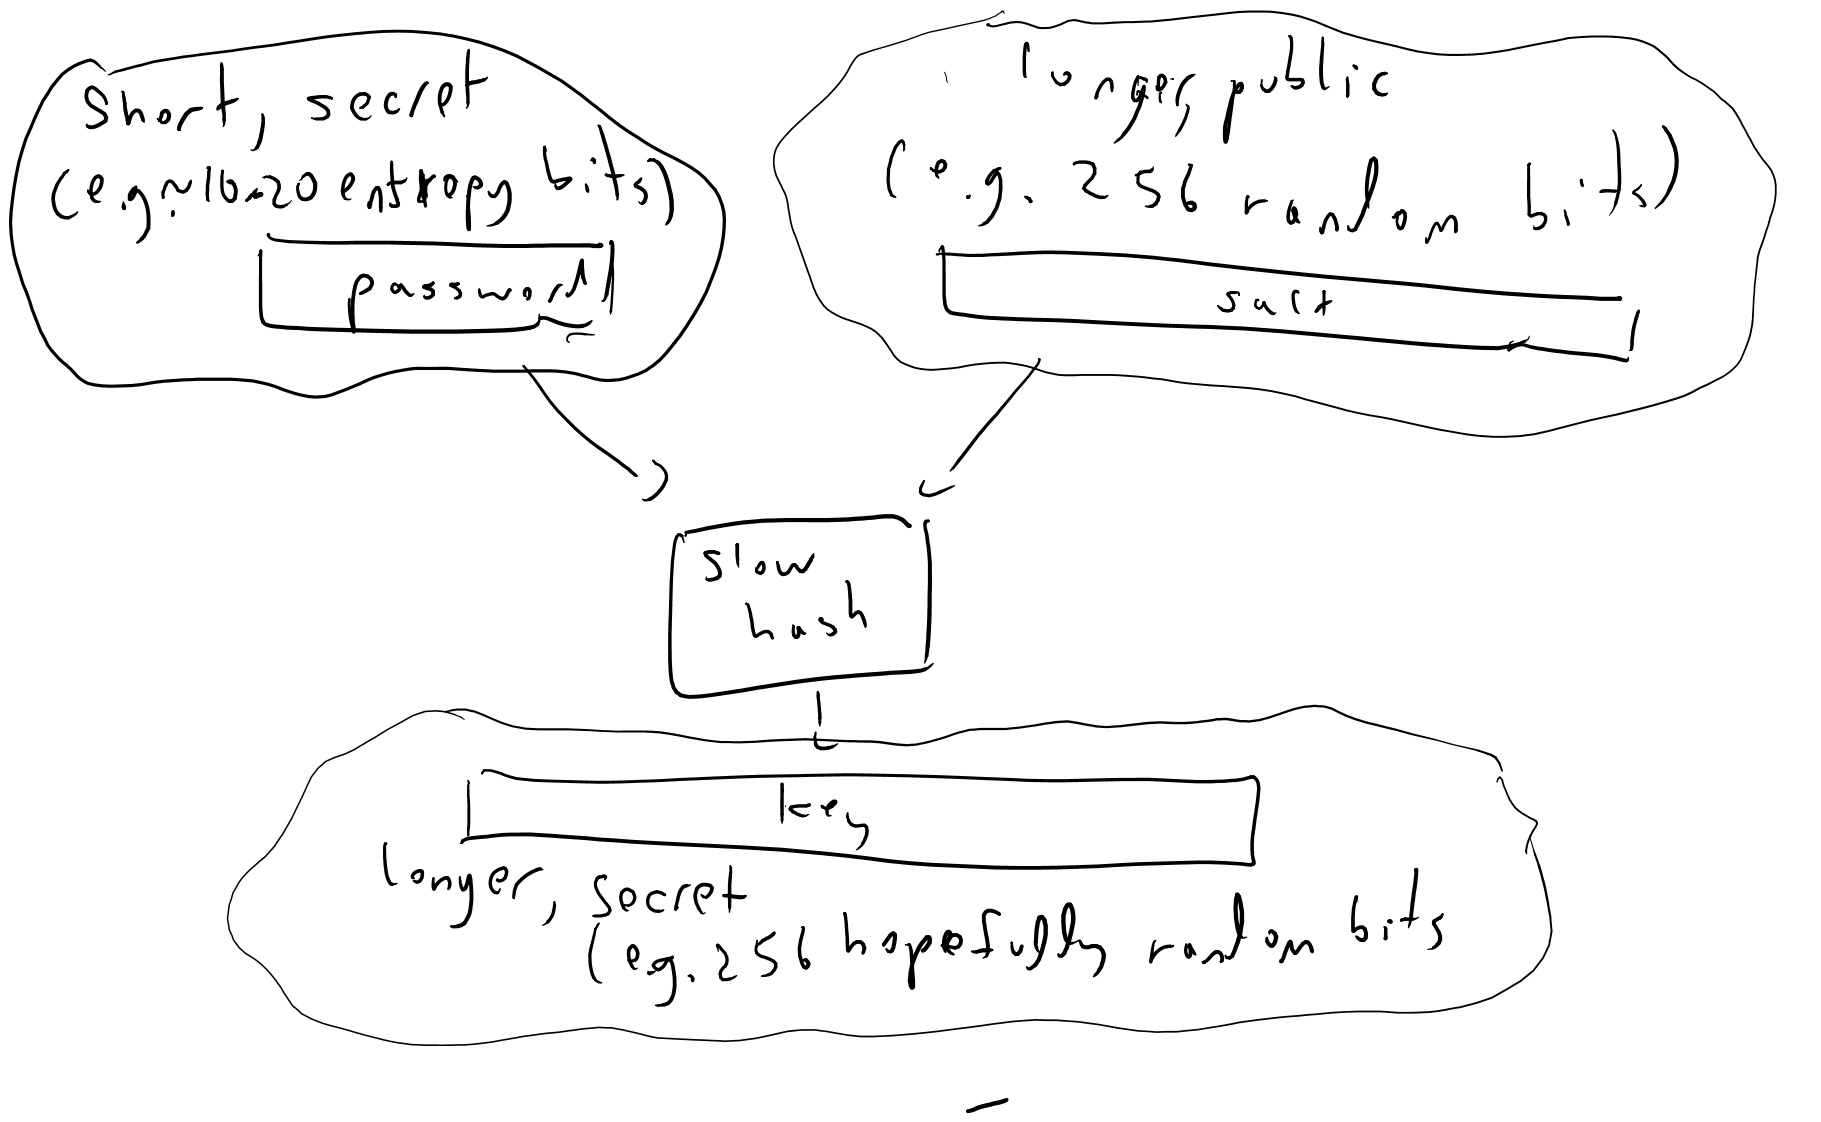
\includegraphics[width=\textwidth, height=0.25\paperheight, keepaspectratio]{../figure/hash-password.jpg}
\caption{To obtain a key from a password we will typically use a
``slow'' hash function to map the password and a unique-to-user public
``salt'' value to a cryptographic key. Even with such a procedure, the
resulting key cannot be consider as secure and unpredictable as a key
that was chosen truly at random, especially if we are in a setting where
an adversary can launch an \emph{offline} attack to guess all
possibilities.}
\label{saltfig}
\end{figure}

Even when we don't use one password to encrypt others, it is generally
considered the best practice to \emph{never} store a password in the
clear but always in this ``slow hashed and salted'' form, so if the
passwords file falls to the hands of an adversary it will be expensive
to recover them.

\section{Merkle trees and verifying
storage.}\label{Merkle-trees-and-verifyin}

Suppose that you outsource to the cloud storing your huge data file
\(x\in\{0,1\}^N\). You now need the \(i^{th}\) bit of that file and ask
the cloud for \(x_i\). How can you tell that you actually received the
correct bit?

Ralph Merkle came up in 1979 with a clever solution, which is known as
``Merkle hash trees''. The idea is the following (see
\cref{merkletreefig}): suppose we have a collision-resistant hash
function \(h:\{0,1\}^{2n}\rightarrow\{0,1\}^n\), and think of the string
\(x\) as composed of \(t\) blocks of size \(n\). We then hash every pair
of consecutive blocks to transform \(x\) into a string \(x_1\) of
\(t/2\) blocks, and continue in this way for \(\log t\) steps until we
get a single block \(y\in\{0,1\}^n\). (Assume here \(t\) is a power of
two for simplicity, though it doesn't make much difference.)


\begin{figure}
\centering
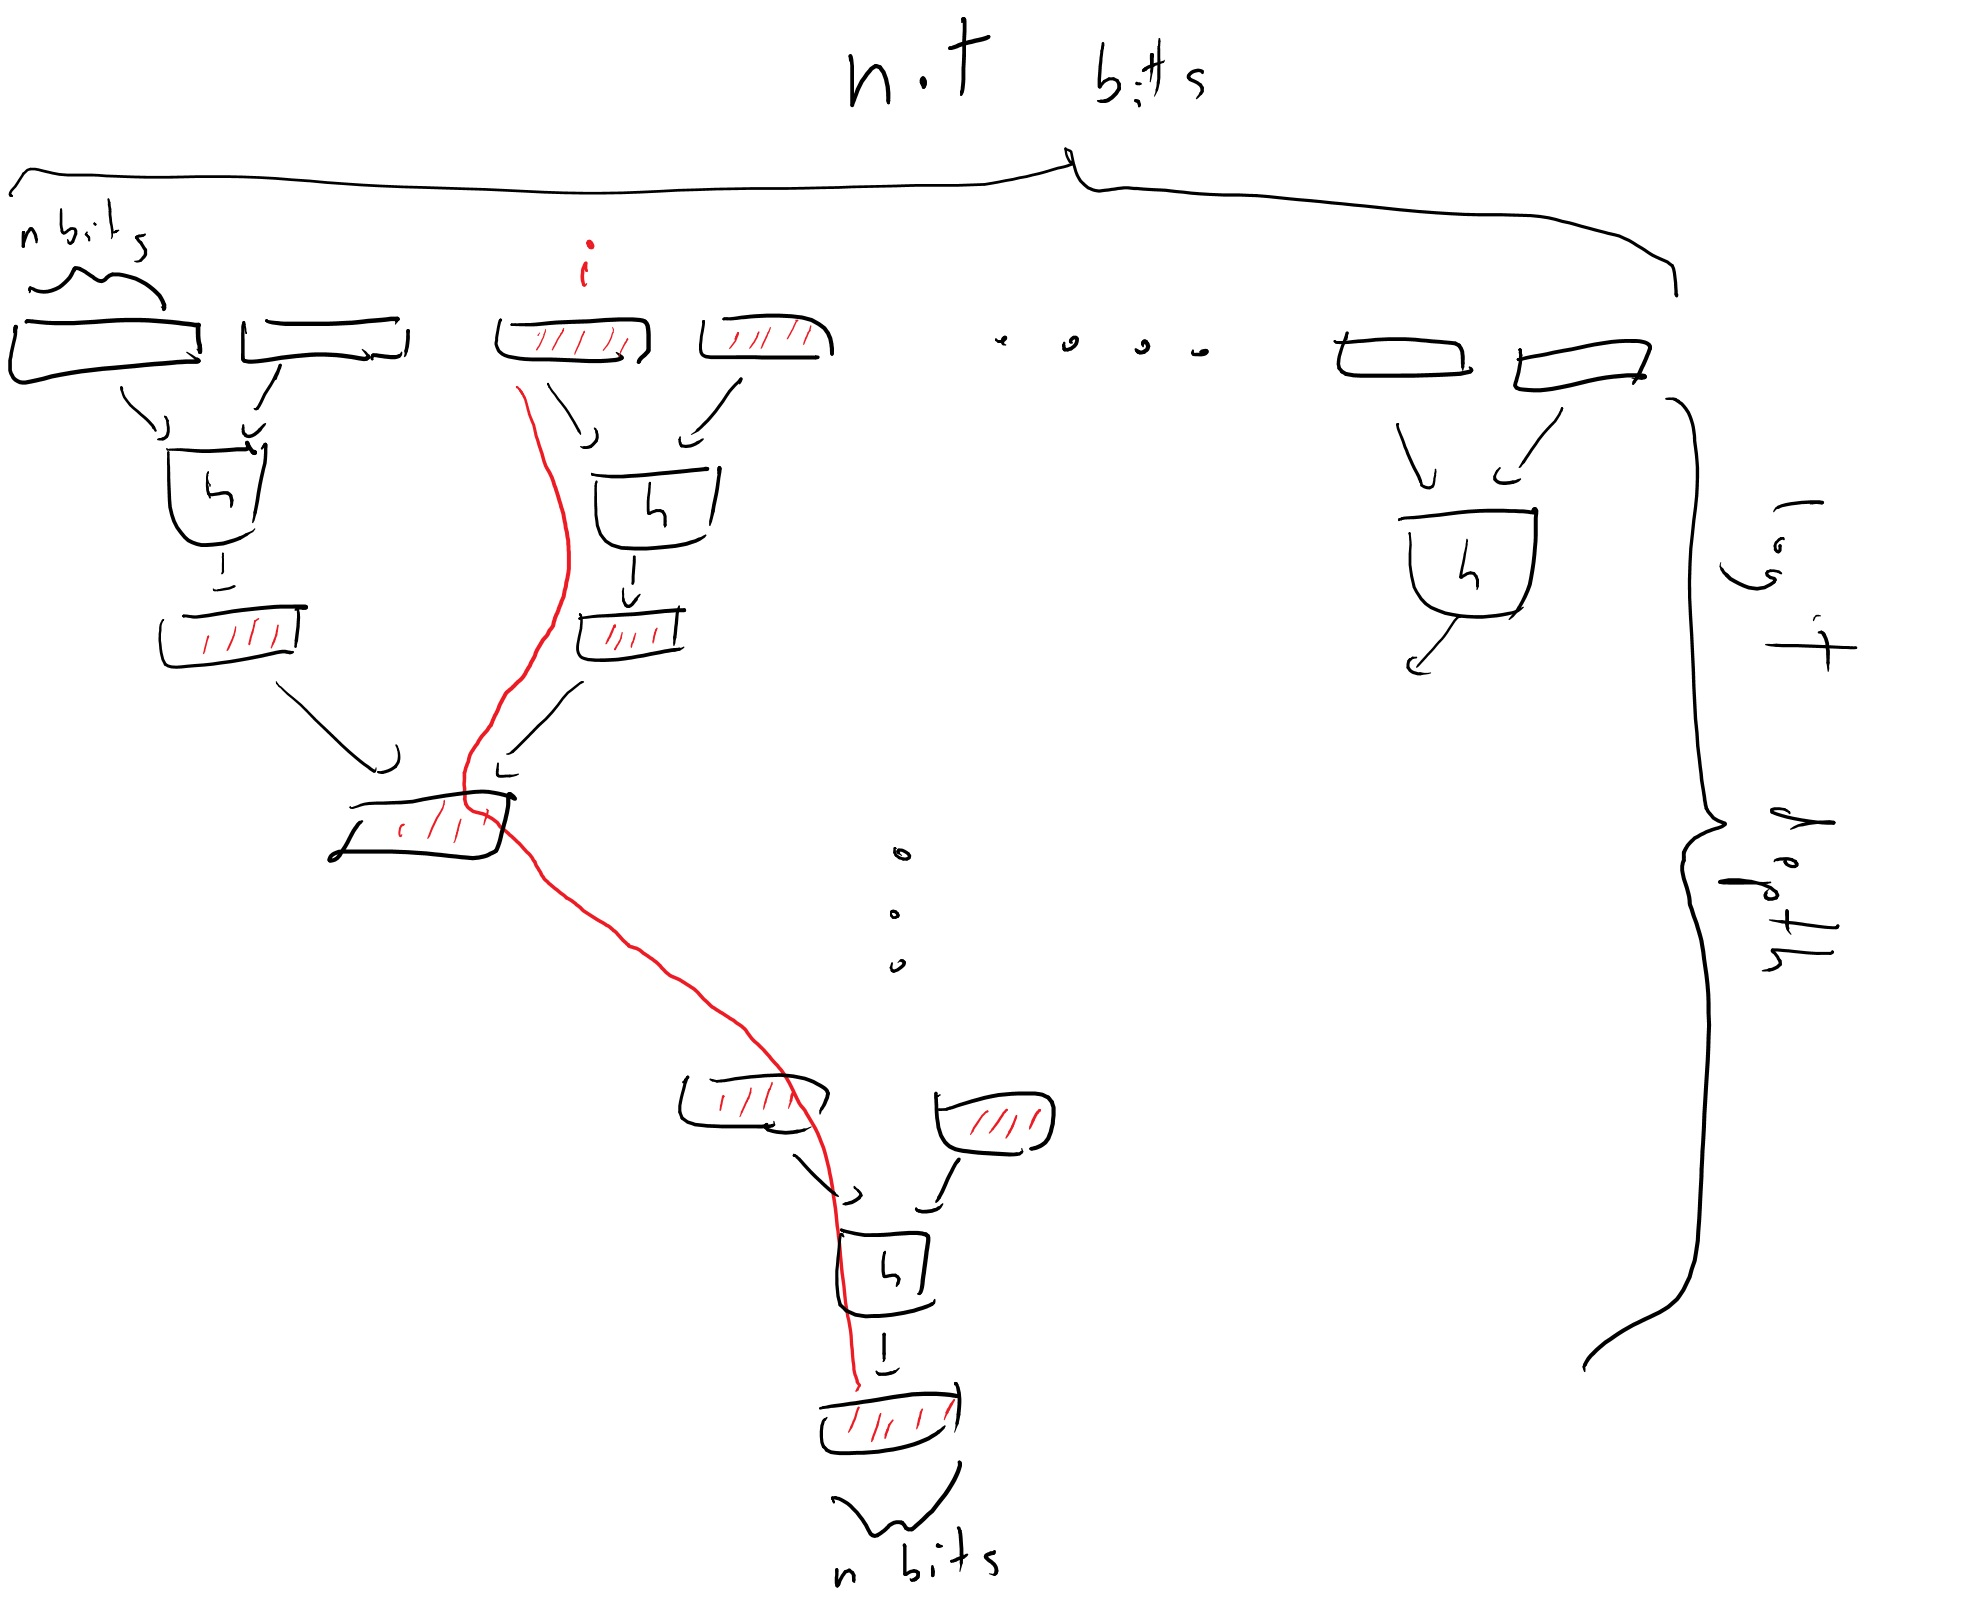
\includegraphics[width=\textwidth, height=0.25\paperheight, keepaspectratio]{../figure/merkle-tree.jpg}
\caption{In the Merkle Tree construction we map a long string \(x\) into
a block \(y\in\{0,1\}^n\) that is a ``digest'' of the long string \(x\).
As in a collision resistant hash we can imagine that this map is ``one
to one'' in the sense that it won't be possible to find \(x'\neq x\)
with the same digest. Moreover, we can efficiently certify that a
certain bit of \(x\) is equal to some value without sending out all of
\(x\) but rather the \(\log t\) blocks that are on the path between
\(i\) to the root together with their ``siblings'' used in the hash
function, for a total of at most \(2\log t\) blocks.}
\label{merkletreefig}
\end{figure}

Alice who sends \(x\) to the cloud Bob will keep the short block \(y\).
Whenever Alice queries the value \(i\) she will ask for a
\emph{certificate} that \(x_i\) is indeed the right value. This
certificate will consists of the block that contains \(i\), as well as
all of the \(2\log t\) blocks that were used in the hash from this block
to the root. The security of this scheme follows from the following
simple theorem:

\hypertarget{merkletreefig}{}
\begin{theorem}[Merkle Tree security] \label[theorem]{merkletreefig}

Suppose that \(\pi\) is a valid certificate that \(x_i=b\), then either
this statement is true, or one can efficiently extract from \(\pi\) and
\(x\) two inputs \(z\neq z'\) in \(\{0,1\}^{2n}\) such that
\(h(z)=h(z')\).

\end{theorem}

\begin{proof} \label[proof]{The-certificate-pi-consis}

The certificate \(\pi\) consists of a sequence of \(\log t\) pairs of
size-\(n\) blocks that are obtained by following the path on the tree
from the \(i^{th}\) coordinate of \(x\) to the final root \(y\). The
last pair of blocks is the a preimage of \(y\) under \(h\), while each
pair on this list is a preimage of one of the blocks in the next pair.
If \(x_i \neq b\), then the first pair of blocks cannot be identical to
the pair of blocks of \(x\) that contains the \(i^{th}\) coordinate.
However, since we know the final root \(y\) is identical, if we compare
the corresponding path in \(x\) to \(\pi\), we will see that at some
point there must be an input \(z\) in the path from \(x\) and a distinct
input \(z'\) in \(\pi\) that hash to the same output.

\end{proof}

\section{Proofs of Retrievability}\label{Proofs-of-Retrievability}

The above provides a way to ensure Alice that the value retrieved from a
cloud storage is correct, but how can Alice be sure that the cloud
server still stores the values that she \emph{did not} ask about?

A priori, you might think that she obviously can't. If Bob is lazy, or
short on storage, he could decide to store only some small fraction of
\(x\) that he thinks Alice is more likely to query for. As long as Bob
wasn't unlucky and Alice doesn't ask these queries, then it seems Bob
could get away with this. In a \emph{proof of retrievability}, first
proposed by Juels and Kalisky in 2007, Alice would be able to get
convinced that Bob does in fact store her data.

First, note that Alice can guarantee that Bob stores at least 99 percent
of her data, by periodically asking him to provide answers (with
proofs!) of the value of \(x\) at 100 or so random locations. The idea
is that if bob dropped more than 1 percent of the bits, then he'd be
very likely to be caught ``red handed'' and get a question from Alice
about a location he did not retain.

Now, if we used some redundancy to store \(x\) such as the RAID format,
where it is composed of some small number \(c\) parts and we can recover
any bit of the original data as long as at most one of the parts were
lost, then we might hope that even if 1\% of \(x\) \emph{was} in fact
lost by Bob, we could still recover the whole string. This is not a
fool-proof guarantee since it could possibly be that the data lost by
Bob was not confined to a single part. To handle this case one needs to
consider generalizations of RAID known as ``local reconstruction codes''
or ``locally decodable codes''. The paper by
\href{http://www.people.seas.harvard.edu/~salil/research/PoR-tcc09.pdf}{Dodis,
Vadhan and Wichs} is a good source for this; see also
\href{http://research.microsoft.com/en-us/um/people/senyk/slides/pos-cai.pdf}{these
slides by Seny Kamara} for a more recent overview of the theory and
implementations.

\section{Entropy extraction}\label{Entropy-extraction}

As we've seen time and again, \emph{randomness} is crucial to
cryptography. But how \emph{do} we get these random bits we need? If we
only have a small number \(n\) of random bits (e.g., \(n=128\) or so)
then we can expand them to as large a number as we want using a
pseudorandom generator, but where do we get those initial \(n\) bits
from?

The approach used in practice is known as ``harvesting entropy''. The
idea is that we make great many measurements \(x_1,\ldots,x_m\) of
events that are considered ``unpredictable'' to some extent, including
mouse movements, hard-disk and network latency, sources of noise
etc\ldots{} and accumulate them in an entropy ``pool'' which would
simply be some memory array. When we estimate that we have accumulated
more than \(128\) bits of randomness, then we hash this array into a
\(128\) bit string which we'll use as a seed for a pseudorandom
generator (see \cref{entropyextfig}).\footnote{The reason that people
  use entropy ``pools'' rather than simply adding the entropy to the
  generator's state as it comes along is that the latter alternative
  might be insecure. Suppose that initial state of the generator was
  known to the adversary and now the entropy is ``trickling in'' one bit
  at a time while we continuously use the generator to produce outputs
  that can be observed by the adversary. Every time a new bit of entropy
  is added, the adversary now has uncertainty between two potential
  states of the generator, but once an output is produced this
  eliminates this uncertainty. In contrast, if we wait until we
  accumulate, say, 128 bits of entropy, then now the adversary will have
  \(2^{128}\) possible state options to consider, and it could be
  computationally infeasible to cull them using further observation.}
Because entropy needs to be measured \emph{from the point of view of the
attacker}, this ``entropy estimation'' routine is a bit of a ``black
art'' and there isn't a very principled way to perform it. In practice
people try to be very conservative (e.g., assume that there is only one
bit of entropy for 64 bits of measurements or so) and hope for the best,
which often works but sometimes also
\href{https://factorable.net/paper.html}{spectacularly fails},
especially in embedded systems that do not have access to many of these
sources.


\begin{figure}
\centering
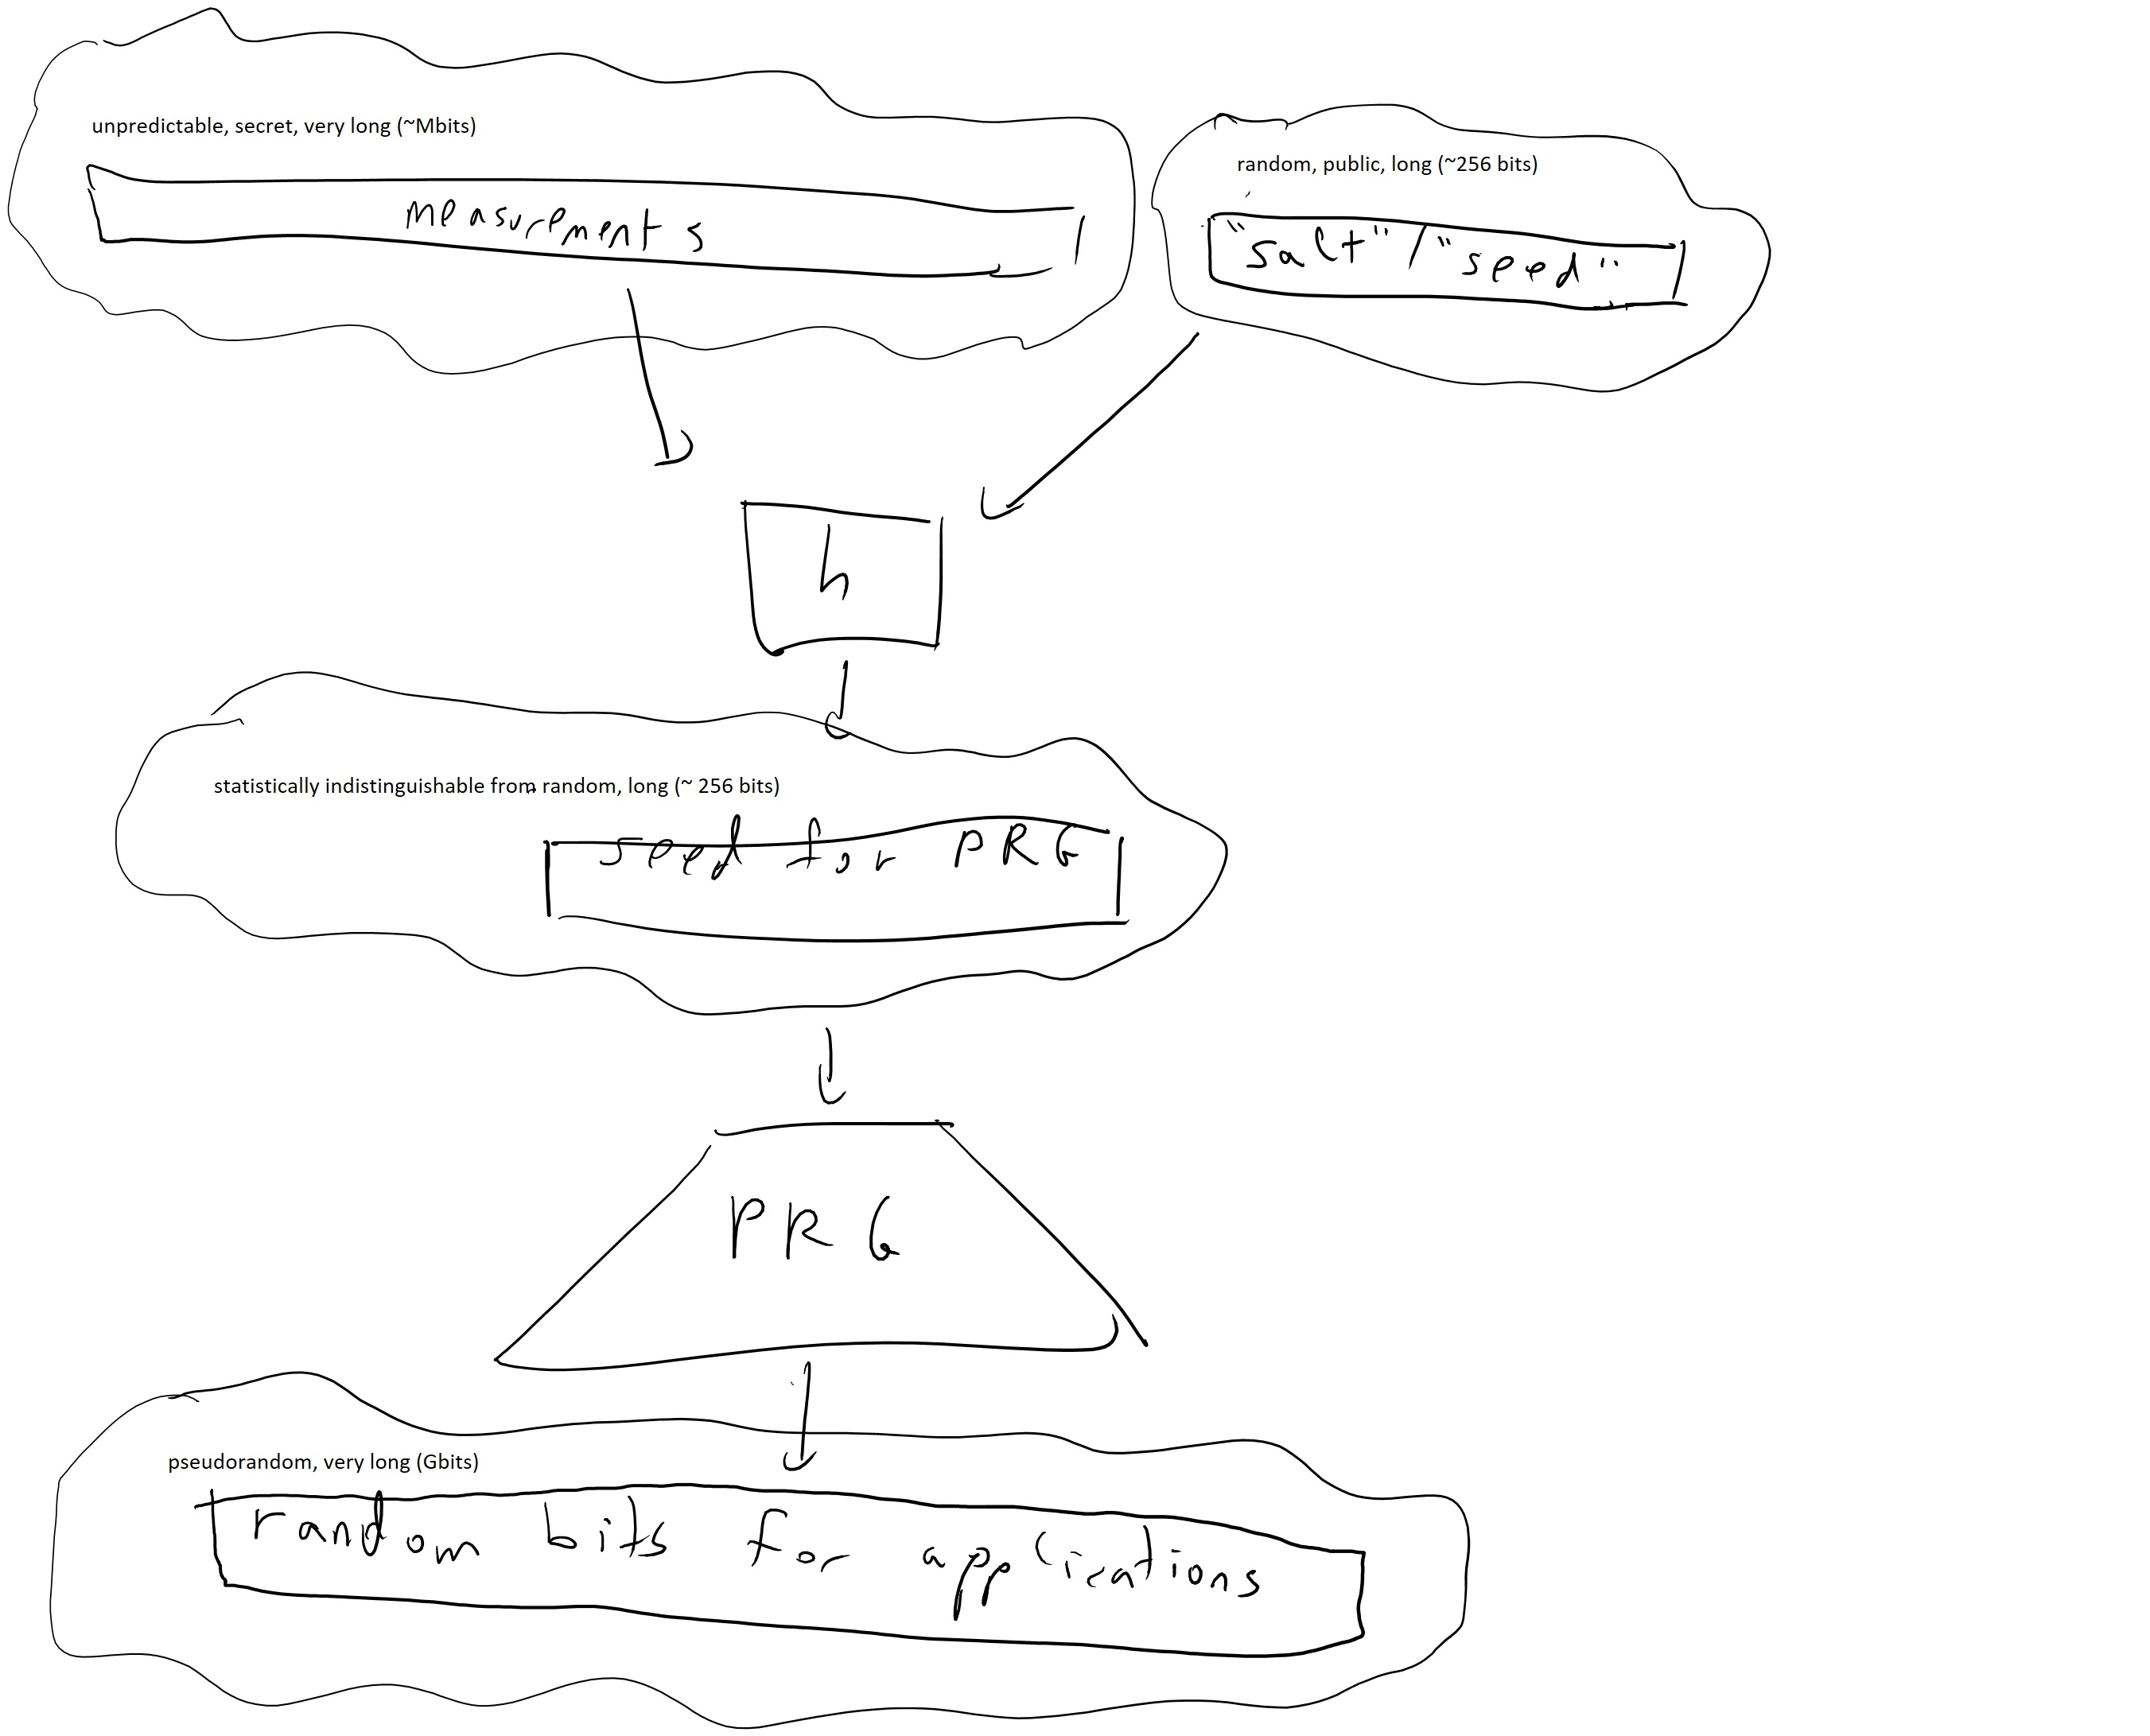
\includegraphics[width=\textwidth, height=0.25\paperheight, keepaspectratio]{../figure/extraction.jpg}
\caption{To obtain pseudorandom bits for cryptographic applications we
hash down measurements which contain some \emph{entropy} in them to a
shorter string that is hopefully truly uniformly random or at least
statistically close to it, and then expand this to get as many
pseudorandom bits as we need using a pseudorandom generator.}
\label{entropyextfig}
\end{figure}

How do hash functions figure into this? The idea is that if an input
\(x\) has \(n\) bits of entropy then \(h(x)\) would still have the same
bits of entropy, as long as its output is larger than \(n\). In practice
people use the notion of ``entropy'' in a rather loose sense, but we
will try to be more precise below.

The \emph{entropy} of a distribution \(D\) is meant to capture the
amount of ``uncertainty'' you have over the distribution. The canonical
example is when \(D\) is the uniform distribution over \(\{0,1\}^n\), in
which case it has \(n\) bits of entropy. If you learn a single bit of
\(D\) then you reduce the entropy by one bit. For example, if you learn
that the \(17^{th}\) bit is equal to \(0\), then the new conditional
distribution \(D'\) is the uniform distribution over all strings in
\(x\in\{0,1\}^n\) such that \(x_{17}=0\) and has \(n-1\) bits of
entropy. Entropy is invariant under permutations of the sample space,
and only depends on the vector of probabilities, and thus for every set
\(S\) all notions of entropy will give \(\log_2 |S|\) bits of entropy
for the uniform distribution over \(S\). A distribution that is uniform
over some set \(S\) is known as a \emph{flat} distribution.

Where different notions of entropy begin to differ is when the
distributions are not flat. The \emph{Shannon entropy} follows the
principle that ``original uncertainty = knowledge learned + new
uncertainty''. That is, it obeys the \emph{chain rule} which is that if
a random variable \((X,Y)\) has \(n\) bits of entropy, and \(X\) has
\(k\) bits of entropy, then after learning \(X\) on average \(Y\) will
have \(n-k\) bits of entropy. That is,

\(H_{Shannon}(X)+H_{Shannon}(Y|X) = H_{Shannon}(X,Y)\)

Where the entropy of a conditional distribution \(Y|X\) is simply
\(\E_{x\leftarrow X} H_{Shannon}(Y|X=x)\) where \(Y|X=x\) is the
distribution on \(Y\) obtained by conditioning on the event that
\(X=x\).

If \((p_1,\ldots,p_m)\) is a vector of probabilities summing up to \(1\)
and let us assume they are rounded so that for every \(i\),
\(p_i = k_i/2^n\) for some integer \(k_i\). We can then split the set
\(\{0,1\}^n\) into \(m\) disjoint sets \(S_1,\ldots,S_m\) where
\(|S_i|=k_i\), and consider the probability distribution \((X,Y)\) where
\(Y\) is uniform over \(\{0,1\}^n\), and \(X\) is equal to \(i\)
whenever \(Y\in S_i\). Therefore, by the principles above we know that
\(H_{Shannon}(X,Y)=n\) (since \(X\) is completely determined \(Y\) and
hence \((X,Y)\) is uniform over a set of \(2^n\) elements), and
\(H(Y|X)=\log k_i\). Thus the chain rule tells us that
\(H_{Shannon}(X) = n - \E[Y|X] = n - \sum_{i=1}^m p_i k_i = \sum_{i=1}^m p_i \log(p_i)\)
since \(p_i = k_i/2^n\) and hence \(\log(p_i)=\log(k_i)-n\).

The Shannon entropy has many attractive properties, but it turns out
that for cryptographic applications, the notion of \emph{min entropy} is
more appropriate. For a distribution \(X\) the \emph{min-entropy} is
simply defined as \(H_{\infty}(X)= \min_x \log(1/\Pr[X=x])\).\footnote{The
  notation \(H_{\infty}(\cdot)\) for min entropy comes from the fact
  that one can define a \href{https://goo.gl/HvVgu1}{\emph{family}} of
  entropy like functions, containing a function for every non-negative
  number \(p\) based on the \(p\)-norm of the probability distribution.
  That is, the Rényi entropy of order \(p\) is defined as
  \(H_p(X)=(1-p)^{-1}\log(\sum_x \Pr[X=x]^p)\). The min entropy can be
  thought of as the limit of \(H_p\) when \(p\) tends to infinity while
  the Shannon entropy is the limit as \(p\) tends to \(1\). The entropy
  \(H_2(\cdot)\) is related to the \emph{collision probability} of \(X\)
  and is often used as well. The min entropy is the smallest among all
  the entropies and hence it is the most \emph{conservative} (and so
  appropriate for usage in cryptography). For \emph{flat sources}, which
  are uniform over a certain subset, all entropies coincide.} Note that
if \(X\) is flat then \(H_{\infty}(X)=H_{Shannon}(X)\) and that
\(H_{\infty}(X) \leq H_{Shannon}(X)\) for all \(X\). We can now formally
define the notion of an extractor:

\hypertarget{extractordef}{}
\begin{definition}[Randomness extractor] \label[definition]{extractordef}

A function \(h:\{0,1\}^{\ell+n}\rightarrow\{0,1\}^n\) is a
\emph{randomness extractor} (``extractor'' for short) if for every
distribution \(X\) over \(\{0,1\}^\ell\) with min entropy at least
\(2n\), if we pick \(s\) to be a random ``salt'', the distribution
\(h(X)\) is computationally indistinguishable from the uniform
distribution.\footnote{The pseudorandomness literature studies the
  notion of extractors much more generally and consider all possible
  variations for parameters such as the entropy requirement, the salt
  (more commonly known as seed) size, the distance from uniformity, and
  more. The type of notion we consider here is known in that literature
  as a ``strong seeded extractor''. See
  \href{https://goo.gl/XHQjTB}{Vadhan's monograph} for an in-depth
  treatment of this topic.}

\end{definition}

The idea is that we apply the hash function to our measurements in
\(\{0,1\}^\ell\) then if those measurements had at least \(k\) bits of
entropy (with some extra ``security margin'') then the output \(h(X)\)
will be as good as random. Since the ``salt'' value \(s\) is not secret,
it can be chosen once at random and hardwired into the description of
the function. (Indeed in practice people often do not explicitly use
such a ``salt'', but the hash function description contain some
parameters IV that play a similar role.)

\hypertarget{randomextractorthm}{}
\begin{theorem}[Random function is an extractor] \label[theorem]{randomextractorthm}

Suppose that \(h:\{0,1\}^{\ell+n}\rightarrow\{0,1\}^n\) is chosen at
random, and \(\ell < n^{100}\). Then with high probability \(h\) is an
extractor.

\end{theorem}

\begin{proof} \label[proof]{Let-h-be-chosen-as-above-}

Let \(h\) be chosen as above, and let \(X\) be some distribution over
\(\{0,1\}^\ell\) with \(\max_x \{ \Pr[X=x]\} \leq 2^{-2n}\). Now, for
every \(s\in\{0,1\}^n\) let \(h_s\) be the function that maps
\(x\in\{0,1\}^\ell\) to \(h(s\|x)\), and let \(Y_s = h_s(X)\). We want
to prove that \(Y_s\) is pseudorandom. We will use the following claim:

\textbf{Claim:} Let \(Col(Y_s)\) be the probability that two independent
sample from \(Y_s\) are identical. Then with probability at least
\(0.99\), \(Col(Y_s) < 2^{-n} + 100\cdot 2^{-2n}\).

\textbf{Proof of claim:}
\(\E_s Col(Y_s) =\sum_s 2^{-n} \sum_{x,x'} \Pr[X=x]\Pr[X=x']\sum_{y\in\{0,1\}^n}\Pr[h(s,x)=y]\Pr[h(s,x')=y]\).
Let's separate this to the contribution when \(x=x'\) and when they
differ. The contribution from the first term is
\(\sum_s 2^{-n}\sum_x \Pr[X=x]^2\) which is simply
\(Col(X)=\sum\Pr[X=x]^2 \leq 2^{-{2n}}\) since \(\Pr[X=x]\leq 2^{-2n}\).
In the second term, the events that \(h(s,x)=y\) and \(h(s,x')=y\) are
independent, and hence the contribution here is at most
\(\sum_{x,x'}\Pr[X=x]\Pr[X=x']2^{-n}\). The claim follows from Markov.

Now suppose that \(T\) is some efficiently computable function from
\(\{0,1\}^n\) to \(\{0,1\}\), then by Cauchy-Schwarz
\(|\E[T(U_n)] - \E[T(Y_s)]| = |\sum_{y\in\{0,1\}^n} T(y)[2^{-n}-\Pr[Y_s=y]]| \leq \sqrt{\sum_y T(y)^2 \cdot \sum_y (2^{-n}-\Pr[Y_s=y])^2 }\)
but opening up \(\sum_y (2^{-n}-\Pr[Y_S=y ])^2\) we get
\(2^{-n} - 2\cdot 2^{-n}\sum_y \Pr[Y_s=y] + \sum_y\Pr[Y_s=y]^2\) or
\(Col(Y_s)-2^{-n}\) which is at most the negligible quantity
\(100\cdot 2^{-2n}\).

\end{proof}

\hypertarget{statextractorrem}{}
\begin{remark}[Statistical randomness] \label[remark]{statextractorrem}

This proof actually proves a much stronger statement. First, note that
we did not at all use the fact that \(T\) is efficiently computable and
hence the distribution \(h_s(X)\) will not be merely pseudorandom but
actually \emph{statistically indistinguishable} from truly random
distribution. Second, we didn't use the fact that \(h\) is completely
random but rather what we needed was merely \emph{pairwise
independence}: that for every \(x\neq x'\) and \(y\),
\(\Pr_s[ h_s(x)=h_s(x')=y] = 2^{-2n}\). There are efficient
constructions of functions \(h(\cdot)\) with this property, though in
practice people still often use cryptographic hash function for this
purpose.

\end{remark}

\subsection{Forward and backward
secrecy}\label{Forward-and-backward-secr}

A cryptographic tool such as encryption is clearly insecure if the
adversary learns the private key, and similarly the output of a
pseudorandom generator is insecure if the adversary learns the seed. So,
it might seem as if it's ``game over'' once this happens. However, there
is still some hope. For example, if the adversary learns it at time
\(t\) but didn't know it before then, then one could hope that she does
not learn the information that was exchanged up to time \(t-1\). This
property is known as ``forward secrecy''. It had recently gained
interest as means to protect against powerful ``attackers'' such as the
NSA that may record the communication transcripts in the hope of
deciphering them in some future after it had learned the secret key. In
the context of pseudorandom generators, one could hope for both forward
and backward secrecy. Forward secrecy means that the state of the
generator is updated at every point in time in a way that learning the
state at time \(t\) does not help in recovering past state, and
``backward secrecy'' means that we can recover from the adversary
knowing our internal state by updating the generator with fresh entropy.
See \href{https://eprint.iacr.org/2005/029}{this paper of me and Halevi}
for some discussions of this issue, as well as
\href{https://eprint.iacr.org/2013/338}{this later work by Dodis et al}.
